\interlude[0]{Safety \& Security \\ \Large \hrule \vspace{1.2em} Kulturelle Aspekte}
\section{Safety \& Security}


\SetNextBackground{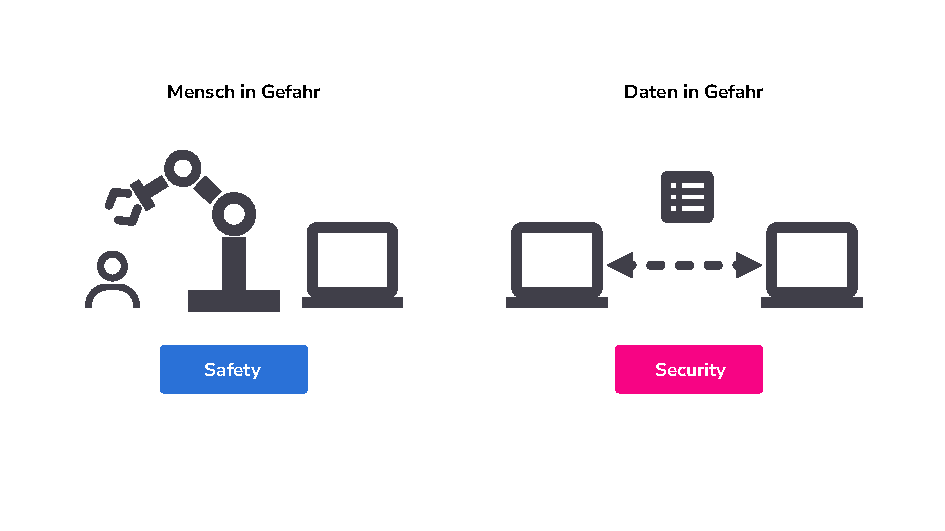
\includegraphics[width=\paperwidth,page=1]{hpke-slide-designs-2024-05-09}}
\begin{frame}[T]{Safety \& Security in Computersystemen}
% GOAL Beide Begriffe einführen
%\small
%% TODO Grafik einfügen
%  \begin{columns}[t,fullwidth]
%   \hfill
%    \begin{column}{.45\linewidth}
%      \begin{block}{Safety}
%      \begin{itemize}
%        \item Schutz von Lebewesen
%      \end{itemize}
%      \end{block}
%    \end{column}
%    \hfill
%    \begin{column}{.45\linewidth}
%      \begin{block}{Security}
%      \begin{itemize}
%        \item Schutz von Informationen
%        \begin{itemize}
%          \item Information vor Dritten geheimhalten
%          \item Information vor Manipulation durch Dritte schützen
%        \end{itemize}
%      \end{itemize}
%      \end{block}
%    \end{column}
%    \hfill
%  \end{columns}
\end{frame}

\begin{frame}[T]{Problemstellungen \& Rahmenbedingungen}
% GOAL Verfahren sind beim ersten Hinblick inkompatibel, Klar machen, dass beide Begriff verschieden sind und verschiedene Vorgehen erfordern
\small

	\begin{tabular}{lllll}
                               & \textbf{Safety}              & \textbf{Security}              \\[1.4em]

  \arrayrulecolor{lightgray}
  \textbf{Fehlerauftreten}     & Zufällig                     & Gezielt (durch Angreifer)      \\[0.35em]
  \midrule                                                                                     \\[-0.75em]
	\textbf{Fehlerbehandlung}    & Weiterbetrieb notwendig      & System stoppen                 \\[0.35em]
  \midrule                                                                                     \\[-0.75em]
  \textbf{Zieldefinition}      & Stabil (Physik bleibt gleich) & In Bewegung (Angreifer lernen)  \\[0.35em]
  \midrule                                                                                     \\[-0.75em]
	\textbf{Abgehangene Sofware} & Stabil!                      & Unsicher?                      \\[0.35em]
  \midrule                                                                                     \\[-0.75em]
	\textbf{Validierungsprozess} & Normiert                     & Dynamisch                      \\
	                             &                              &
	\end{tabular}

  % OLD slide with two-column bullet points
  % \begin{columns}[t,fullwidth]
  %  \hfill
  %   \begin{column}{.45\linewidth}
  %     \begin{block}{Safety}
  %     \begin{itemize}
  %       \item Fehler: Zufällig
  %       \item Im Fehlerfall: Weiterbetrieb ermöglichen!
  %       \item Stabile Zieldefinition:\\Physik bleibt gleich
  %       \item Abgehangene Software $\rightarrow$ Stabil!
  %       \item Normierte Validierungsprozesse
  %     \end{itemize}
  %     \end{block}
  %   \end{column}
  %   \hfill
  %   \begin{column}{.45\linewidth}
  %     \begin{block}{Security}
  %     \begin{itemize}
  %       \item Fehler: Gezielt durch Angreifer
  %       \item Im Fehlerfall: Lieber das System stoppen
  %       \item Zieldefinition ist in Bewegung:\\Angreifer lernen dazu
  %       \item Abgehangene Software $\rightarrow$ Unsicher?
  %       \item Dynamische Validierungsprozesse
  %     \end{itemize}
  %     \end{block}
  %   \end{column}
  %   \hfill
  % \end{columns}
\end{frame}


\begingroup
\ExplSyntaxOn
\definecolor{green1}{RGB}{48, 175, 155}
\definecolor{green2}{RGB}{130, 221, 207}
\colorlet{green3}{rosenpass-lightblue}
\newcommand*{\Level}[1]{

	\str_case:nnF {#1} {
		{+}{
      \begin{tikzpicture}[/tikzsymbolsstyle]
        \draw[fill=green3] (0,0) circle [radius=0.21];
      \end{tikzpicture}%
    }
		{++}{
      \begin{tikzpicture}[/tikzsymbolsstyle]
        \draw[fill=green2] (0,0) circle [radius=0.21];
      \end{tikzpicture}%
    }
		{+++}{
      \begin{tikzpicture}[/tikzsymbolsstyle]
        \draw[fill=green1] (0,0) circle [radius=0.21];
      \end{tikzpicture}%
    }
		{-}{-}
	}
	{#1}
}
\ExplSyntaxOff

\begin{frame}[T]{Vertrauen schaffen: Akzeptanzkriterien}
  % GOAL erklären, wie man in Safety/Security Konfidenz erzeugt, einen guten Job gemacht zu haben
%  \begin{table}[]
    \begin{tabular}{lrlrl}
      \multirow{2}{*}{}
                          & \multicolumn{2}{c}{\bfseries Safety} & \multicolumn{2}{c}{\bfseries Security} \\[0.2em]
                          &      Konfidenz     &  Verbreitung    &  Konfidenz          &  Verbreitung     \\[0.9em]

    \arrayrulecolor{lightgray}

    Praktische Tests      & \Level{+++}    & \Level{+++}     & \Level{+}           & \Level{++}           \\[-0.10em]
    \midrule                                                                                              \\[-1.20em]
    Proven-in-use         & \Level{++}     & \Level{+}       & \Level{-}           & \Level{+}            \\[-0.10em]
    \midrule                                                                                              \\[-1.20em]
    Mathematische Beweise & \Level{+++}    & \Level{-}       & \Level{+++}         & \Level{++}           \\[-0.10em]
    \midrule                                                                                              \\[-1.20em]
    Externe Audits        & \Level{++}     & \Level{+++}     & \Level{+++}         & \Level{+++}          \\[-0.10em]
    \end{tabular}
    \\[1em]
    \textbf{Verbreitung} Häufigkeit als tragendes Argument im Assurance-Case\\
    \textbf{Konfidenz} Vertrauen in das Kriterium


  % \begin{itemize}
  %   \item Safety
  %   \begin{itemize}
  %     \item Goldstandard: Requirements-getriebenes Testen % üblich
  %     \item Alternative: "Proven in use" % unüblich
  %     \item Alternative: Formale Verifikation % selten
  %   \end{itemize}

  %   \item Security
  %   \begin{itemize}
  %     \item "Proven in use" reicht nicht, aber neuen Verfahren wird dennoch misstraut
  %     \item Testen unzureichend, aufgrund gezielter Angriffe
  %     \item Formale Verifikation ist der Goldweg
  %   \end{itemize}
  % \end{itemize}

\end{frame}
\endgroup

\begin{frame}[T]{Ingenieurskulturen}
  % GOAL Es gibt Unterschiede, die Begründet sind. Wenn Safety und Security verbunden werden sollen, müssen beide Gründe verstanden werden.
	\begin{columns}[t,fullwidth]
		\hfill
		\begin{column}{.45\linewidth}
			\begin{block}{Safety $\Longrightarrow$ Konservativ}
				\begin{itemize}
				\item Menschen Sterben bei Versagen
				\item Probleme sind Verstanden und Stabil
				\end{itemize}
			\end{block}
		\end{column}
		\begin{column}{.45\linewidth}
			\begin{block}{Security $\Longrightarrow$ Progressive}
				\begin{itemize}
				\item Versagen erzeugt eher finanziellen Schaden
				\item Problemtypen sind dynamisch und ändern sich dauernd
				\end{itemize}
			\end{block}
		\end{column}
		\hfill
	\end{columns}

	\hskip.5\LeftSlideIndent
    \begin{block}{Security + Safety $\Longleftrightarrow$ Konservativ $\lightning$ Progressiv}
	    \begin{itemize}
	      \item Menschen sterben bei Versagen
	      \item Probleme sind dynamisch, Zielsetzung in Bewegung
	    \end{itemize}
  	\end{block}
\end{frame}

\begin{frame}[T]{Safety + Security: Checkliste}
  % GOAL Klar machen, dass beide Domänen nicht unversöhnbar sind
  \begin{enumerate}
	% TODO marei smallcaps
	% TODO marei checkbox right aligned after the items, all checkboxes but the last one checked
    \item Hohe Zuverlässigkeit\hfill $[ ]$
    \item Klarheit über Systemziele
    \item Umfassende Validierung
	\item Unabhängiges Review
    \item Analyse von Softwaresystemen in reeller Hardware
    \item Redundante Systeme
    \item \textbf{Kryptoagilität}
  \end{enumerate}
\end{frame}
